\section{Project management method}


With our weekly or biweekly meetings with the customer in mind as well as his request for intermediate prototypes to be presented at these meetings, the choice of scrum with it’s sprints that last as long as these intervals is natural. That as well as everyone on the group having previous experience with the scrum process through other projects.
With our choice of the agile project management method Scrum we had to set up some guidelines for ourselves so we follow the intended process as closely as our project and experience allow. With that said we have defined some changes to the process.


\subsection{Modifications to our project}

To fit with our schedule we will modify the scrum model somewhat. We will move the daily meetings to be three times a week(Monday,Wednesday and Friday) as well as doing work sessions on these days. Sprints will also be modified to primarily be biweekly and may vary between sprints according to our meetings with the customer and as the intermediate prototypes we will present to him are finished. Sprint backlogs will be very crucial for our use. With the abstract goals of the project set forth, the gradual inclusion of new features as we and the customer see the project evolve will be mirrored in the backlogs from sprint to sprint. We will also maintain a product backlog with input from the customer. To properly fit our product goals the differences between faculties of a normal product backlog and the requirements and wishes of the customer we will have to modify the backlog to be somewhat of an intersection between requirements and feature goals. Another important difference to normal scrum evolution will have to be the “definitions of done”. As our end state is diffuse in regards to the tangible product we have in collaboration with the customer some design goals(see requirements) that will be the main focus of our project.


\subsection{Project management tools}


To accompany us in the scrum process we have chosen an online tool called ScrumDo(www.scrumdo.com). This tool has features for most if not all parts of the scrum process. Using this tool consistently will be our main method of maintaining and separating packages from the WBS(Work Breakdown Structure). In the context of ScrumDo and Scrum these low level work packages are called stories and are moved accordingly from "ToDo" over to "In progress" and eventually to "Done


\begin{figure}
	\centering
	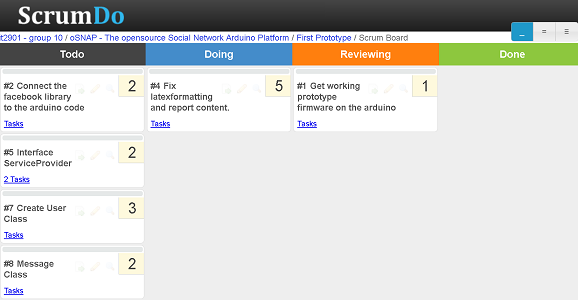
\includegraphics{./img/management-scrumdo.png}
	\caption{The Scrum Board in ScrumDo}
	\label{fig:management-scrumdo}
\end{figure}





Another part of a collaborative project is the software sharing mechanisms. Initially we decided on using GIT, which is an open source distributed revision control system. This differs from the centralised control systems like Subversion and SVN in its complexity and it's capability of handling several "branches" of software. The branches can head in different directions and later be merged instead of always maintaing a central, "correct" version on a server in that all involved have their own revisions locally, but can share to a common version(which also sits locally!). The faculty handed out SVN(Subversion) and TRAC to keep track of our software and we will use these to share finished code for evaluation purposes. We decided to use GIT as our work system because of it's more flexible use and because several of our members had problems getting access to the Subversion servers. 





